% Геометрические примитивы.
\subsection{Геометрические примитивы, используемые в главе}

\subsubsection{Основные понятия}

При рассмотрении геометрических объектов наряду с понятием точки $P = (x, y, z)$ будем использвать также понятие радиус-вектора $\overline{P}$, компонентами которого являются координаты этой точки.
В дальнейшем будем считать эти термины взаимозаменяемыми.

Отрезок с концами $A$, $B$ (с радиус-векторами $\overline{A}$, $\overline{B}$ соотвественно) будем определять как геометрическое место точек\label{term:gmt} (ГМТ\label{abbr:gmt}) $\overline{P}(\alpha)$ в пространстве, заданное следующим образом:
\begin{equation}\label{eqn:text_1_geo_prim_segment}
	\left\{
		\begin{aligned}
			& \overline{P}(\alpha) = \overline{A} + \alpha (\overline{B} - \overline{A}) = \overline{A} + \alpha \overline{AB} \\
			& 0 \le \alpha \le 1
		\end{aligned}
	\right.
\end{equation}

Треугольник с вершинами $A$, $B$, $C$ (с радиус-векторами $\overline{A}$, $\overline{B}$, $\overline{C}$ соответственно) будем определять как ГМТ $\overline{P}(\beta, \gamma)$ в пространстве, заданное следующим образом:
\begin{equation}\label{eqn:text_1_geo_prim_triangle}
	\left\{
		\begin{aligned}
			& \overline{P}(\beta, \gamma) = \overline{A} + \beta (\overline{B} - \overline{A}) + \gamma (\overline{C} - \overline{A}) = \overline{A} + \beta \overline{AB} + \gamma \overline{AC} \\
			& \beta \ge 0 \\
			& \gamma \ge 0 \\
			& \beta + \gamma \le 1
		\end{aligned}
	\right.
\end{equation}

Прямоугольный параллелепипед будем определять как ГМТ $\overline{P} = (x, y, z)$ в пространстве, удовлетворяющих следующей системе неравенств:
\begin{equation}\label{eqn:text_1_geo_prim_parallelepiped}
	\left\{
		\begin{aligned}
			& x_l \le x \le x_h \\
			& y_l \le y \le y_h \\
			& z_l \le z \le z_h
		\end{aligned}
	\right.
\end{equation}

\begin{definition}
Пусть дано некоторое ГМТ $G$, на точках $\overline{P} \in G$ которого определена неотрицательная функция $R: G \rightarrow \mathbb{R}$, $R(\overline{P}) \ge 0$.
Тогда \textbf{оболочкой}\label{term:envelope} $G$, заданной указанной функцией $R(\overline{P})$, будем называть ГМТ, определяемое следующим образом:
\begin{equation}
	O_R(G) = \{ \overline{P}_0: \exists \overline{P} \in G \implies |\overline{P}_0 - \overline{P}| \le R(\overline{P}) \}
\end{equation}
\end{definition}

\subsubsection{Задача о пересечении треугольника и прямоугольного параллелепипеда в пространстве}

Пусть в пространстве определены треугольник согласно \eqref{eqn:text_1_geo_prim_triangle} и прямоугольный параллелепипед согласно \eqref{eqn:text_1_geo_prim_parallelepiped}.
Требуется определить, имеют ли они общие точки.

\begin{figure}[ht]
	\centering
		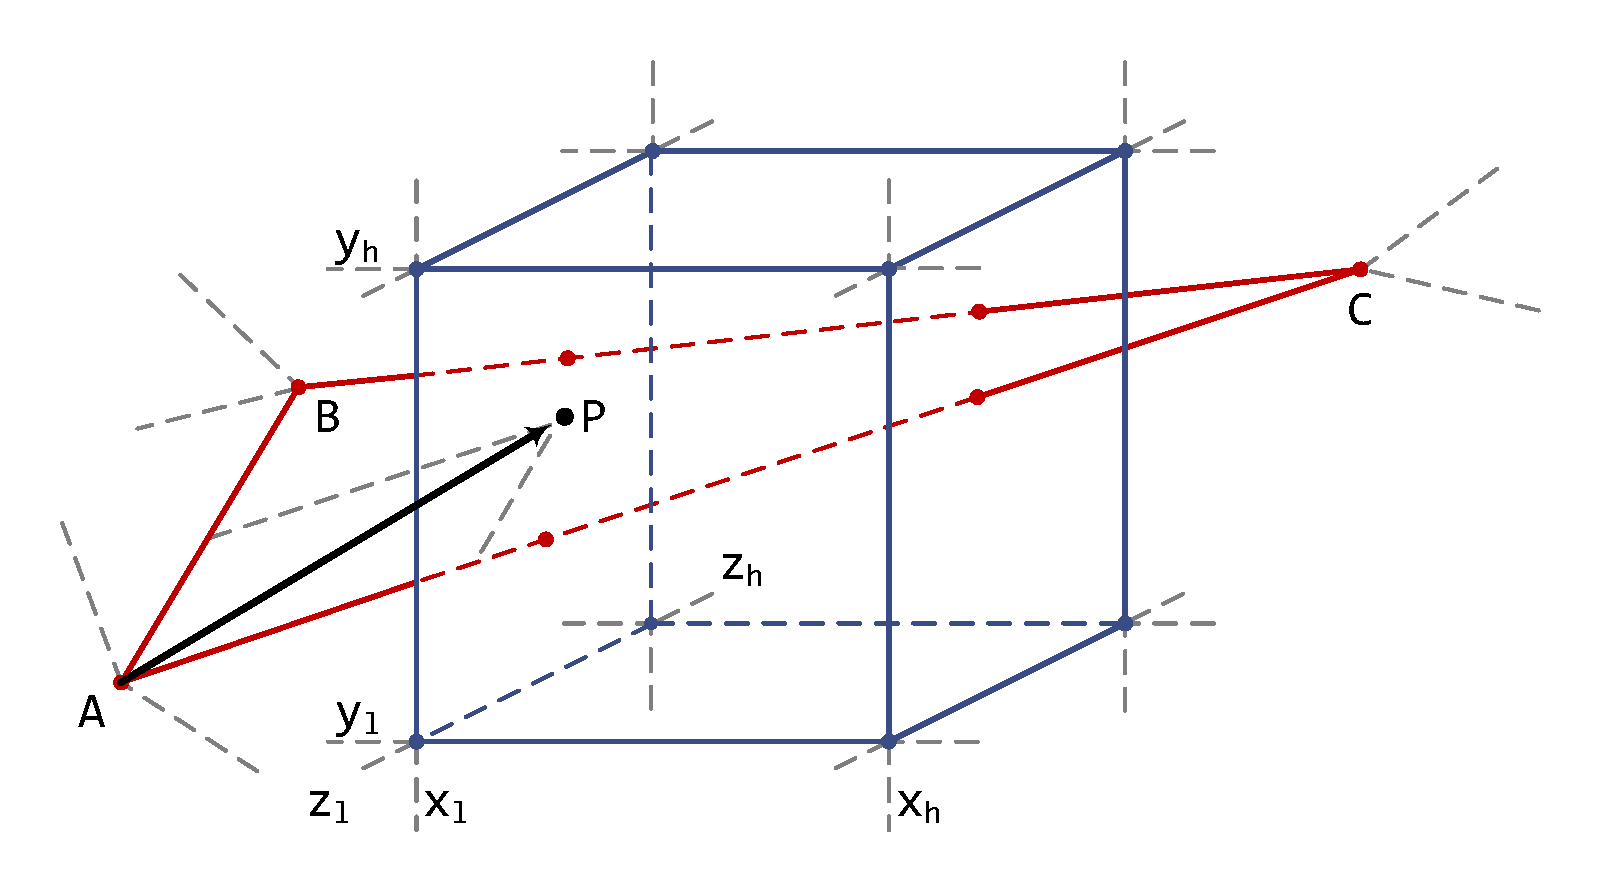
\includegraphics[width=0.80\textwidth]{./pics/text_1_geo_prim/tri_block_intersect.pdf}
	\caption{Пересечение прямоугольного параллелепипеда и треугольника}
	\label{fig:text_1_geo_prim_tri_block_intersect}
\end{figure}

Для решения этой задачи подставим $\overline{P}(\beta, \gamma)$ из \eqref{eqn:text_1_geo_prim_triangle} в систему неравенств \eqref{eqn:text_1_geo_prim_parallelepiped}, получив следующую систему неравенств с двумя переменными $\beta$ и $\gamma$:
\begin{equation}\label{eqn:text_1_geo_prim_1}
	\left\{
		\begin{aligned}
			& x_l \le x_A + \beta (x_B - x_A) + \gamma (x_C - x_A) \le x_h \\
			& y_l \le y_A + \beta (y_B - y_A) + \gamma (y_C - y_A) \le y_h \\
			& z_l \le z_A + \beta (z_B - z_A) + \gamma (z_C - z_A) \le z_h \\
			& \beta \ge 0 \\
			& \gamma \ge 0 \\
			& \beta + \gamma \le 1
		\end{aligned}
	\right.
\end{equation}

Cистема \eqref{eqn:text_1_geo_prim_1} может быть решена методом свертывания конечных систем линейных неравенств \cite{Chernikov1963}.
Для применения метода свертывания систем линейных неравенств неравенства системы \eqref{eqn:text_1_geo_prim_1} необходимо привести к виду $k_{\beta}\beta + k_{\gamma}\gamma + k \le 0$, после чего получим следующую систему неравенств:
\begin{equation}\label{eqn:text_1_geo_prim_2}
	\left\{
		\begin{aligned}
			& (x_B - x_A) \beta + (x_C - x_A) \gamma + (x_A - x_h) \le 0 \\
			& (x_A - x_B) \beta + (x_A - x_C) \gamma + (x_l - x_A) \le 0 \\
			& (y_B - y_A) \beta + (y_C - y_A) \gamma + (y_A - y_h) \le 0 \\
			& (y_A - y_B) \beta + (y_A - y_C) \gamma + (y_l - y_A) \le 0 \\
			& (z_B - z_A) \beta + (z_C - z_A) \gamma + (z_A - z_h) \le 0 \\
			& (z_A - z_B) \beta + (z_A - z_C) \gamma + (z_l - z_A) \le 0 \\
			& -1 \cdot \beta + 0 \cdot \gamma \le 0 \\
			& 0 \cdot \beta + (-1) \cdot \gamma \le 0 \\
			& \beta + \gamma + (-1) \le 0
		\end{aligned}
	\right.
\end{equation}

Cистема неравенств \eqref{eqn:text_1_geo_prim_2} является системой с двумя переменными ($\beta$ и $\gamma$), поэтому после выполнения одного шага свертывания она превратится в систему неравенств с одной переменной.
Деформация системы для исключения из нее переменной $\beta$ выполняется следующим образом.
Составляется новая система неравенств, в которую войдут все неравенства системы \eqref{eqn:text_1_geo_prim_2} вида $k_{\gamma} \gamma + k \le 0$, а каждая пара неравенств
\begin{equation}
	\begin{aligned}
		k_{\beta}^1 \beta + k_{\gamma}^1 \gamma + k^1 \le 0 \\
		k_{\beta}^2 \beta + k_{\gamma}^2 \gamma + k^2 \le 0
	\end{aligned},
\end{equation}

в которой коэффициенты при $\beta$ удовлетворяют неравенствам $k_{\beta}^1 < 0$, $k_{\beta}^2 > 0$, войдет в деформированную систему неравенств в виде
\begin{equation}
	(k_{\gamma}^1 k_{\beta}^2 - k_{\gamma}^2 k_{\beta}^1) \gamma + (k^1 k_{\beta}^2 - k^2 k_{\beta}^1) \le 0. 
\end{equation}

Так как система \eqref{eqn:text_1_geo_prim_2} содержит 9 неравенств, из которых в одном коэффициент при $\beta$ нулевой, не более чем в четырех –- положительный, и не более чем в четырех -- отрицательный, то в результате выполнения деформации получим систему, состоящую не более чем из 17 неравенств.
Если деформированная система неравенств с одной переменной имеет решение, то исходные треугольник и прямоугольный параллелепипед имеют общие точки.

\subsubsection{Задача поиска точек пересечения двух треугольников в пространстве}

